\documentclass[a4paper,12pt,twocolumn]{article}
\usepackage{graphicx,epsfig}
\usepackage{natbib}
\usepackage{hyperref} 
\usepackage{times}
\usepackage[leftcaption]{sidecap}
\usepackage{subfigure}      % figures can have sub chunks
\usepackage{geometry}       % this maxes page usage, making the below unnecessary
\usepackage[cc]{titlepic}   % allows a pic to be included in the title page
\textwidth = 6.75in
\oddsidemargin = -0.25in
\textheight = 10in
\topmargin = -0.5in

\usepackage{fancyhdr}
\pagestyle{fancy}
\lhead{{\it A. Jaamour, A. Lissak}}
\chead{Altruistic Strategies For Colony Growth}
\rhead{CM30229 Coursework 2}
\lfoot{}
\cfoot{\thepage}
\rfoot{}

\newcommand{\goodgap}{
 \hspace{\subfigtopskip}%
 \hspace{\subfigbottomskip}}

\title{Altruistic Strategies For Colony Growth}
\author{Adam Jaamour, Andrea Lissak}
\titlepic{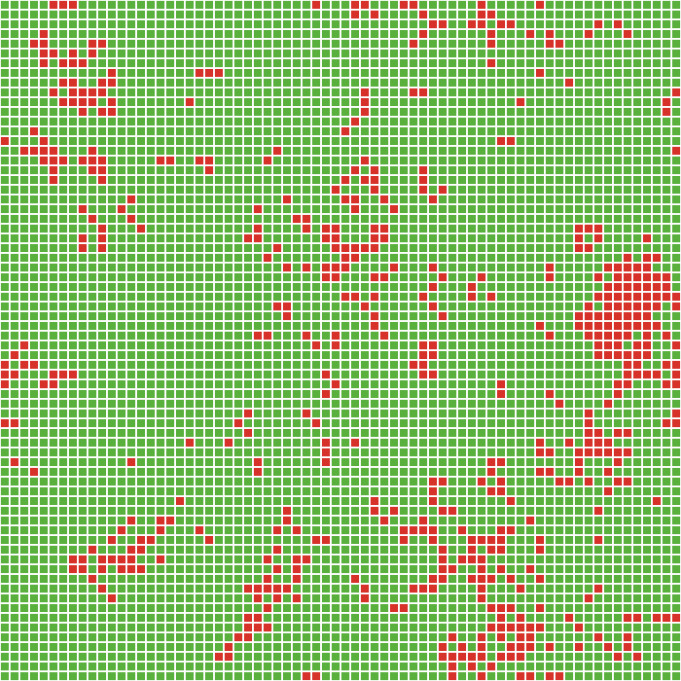
\includegraphics[width=0.5\linewidth]{figures/world.png}}

\renewcommand{\familydefault}{lmss}
%beautiful table
\usepackage[table]{xcolor}
\usepackage{longtable}
\usepackage{tabularx}
%\setlist{nolistsep}
\definecolor{orange}{HTML}{cd8641}
\definecolor{yellow}{HTML}{f0f4b2}
\definecolor{bordeaux}{HTML}{641113}

%%%%%%%%%%%%%%%%%%%%%%%%%%%%%%%%%%%%%%%%%%%%%%%%%%%%%%%%%%%%%%%%%%%%%%%%
%%%%%%%%%%%%%%%%%%%%%%%%%%%%%%%%%%%%%%%%%%%%%%%%%%%%%%%%%%%%%%%%%%%%%%%%
%%%%%%%%%%%%%%%%%%%%%%%%%%%%%%%%%%%%%%%%%%%%%%%%%%%%%%%%%%%%%%%%%%%%%%%%

\begin{document}
\maketitle
\clearpage

\section{Introduction}
\begin{flushleft}
The tested hypothesis is the benefit of altruistic strategies for colony growth. The credit for inspiration goes to \citet{bats}; he revealed how \textit{Vampire Bats} show altruistic behaviour towards other members of the same species who are not strictly related to them. This research is used as proof of altruistic strategies being chosen by natural selection. While the simulation environment used in this report is completely different from the corresponding real world example, the aim of the experiment is to extract variables which affect colony growth, in the context of altruism.
\end{flushleft}
\begin{flushleft}
\citet{dawkins} provides an interesting metaphor for altruistic and selfish behaving entities within a population; the former are called "suckers", the latter "cheats". In the chapter \textit{"You scratch my back, I'll ride on yours"} \cite[p. 165]{dawkins} it is explained how "cheats" can take advantage of "suckers" by simply not returning favours. The ultimate consequence of this scenario is the extinction of altruist behaviour (or its recurring shrinking and expansion).
\end{flushleft}

\begin{flushleft}
The current project shows how altruistic behaviours, like the one described by \citet{bats}, apply when resources are scarce; while "cheats" described by \citet{dawkins} emerge and take over when there are no threats to survival.
\end{flushleft}

%%%%%%%%%%%%%%%%%%%%%%%%%%%%%%%%%%%%%%%%%%%%%%%%%%%%%%%%%%%%%%%%%%%%%%%%
%%%%%%%%%%%%%%%%%%%%%%%%%%%%%%%%%%%%%%%%%%%%%%%%%%%%%%%%%%%%%%%%%%%%%%%%
%%%%%%%%%%%%%%%%%%%%%%%%%%%%%%%%%%%%%%%%%%%%%%%%%%%%%%%%%%%%%%%%%%%%%%%%

\section{Approach}
\begin{flushleft}
While \citet{smaldino} demonstrate that, for certain conditions, cooperative behaviour is worse in harsh environments and better in safe ones, we argue that the opposite might also be the case. We can do this because, as reminded to us by \citet{bryson}, simulations are strictly theoretical and cannot even remotely possibly simulate any kind of realistic real-world situation. So, even just a single heuristic change can flip outcomes.
\end{flushleft}

\begin{flushleft}
We believe we constructed a rational rule-base with respect to simulation of real-world behaviour. More specifically, we introduced just one rule to \citeauthor{smaldino}'s simulation; we will refer to the added rule as \textit{altruistic suicide}. It is intended to be a simplification of any altruistic behaviour happening in nature. The assumption behind it is that any altruistic act, as also clarified by \citet[p. 451]{smaldino}, has the risk of bringing the entity performing it closer to its death. This \textit{altruistic suicide} strategy requires part of the population to die and share its resources (its corpse) with the remaining entities. However, we must clarify that in the simulation, the population is split between defectors (who do not commit \textit{altruistic suicide}) and cooperators (who commit \textit{altruistic suicide}). The important detail here is that the resources resulting from an \textit{altruistic suicide} are only shared with other cooperative, suicidal entities, not with the selfish part of the population.
\end{flushleft}

\begin{flushleft}
This suicidal heuristic was indeed inspired by \citet{bats} and the Vampire Bat's altruistic behaviour.
\end{flushleft}

\begin{flushleft}
The experiment consists in changing two variables: the \textit{cost of living} and the \textit{suicide rate}. Throughout the experiment, the initial consists of 100 agents, divided in 50\% cooperators and 50\% defectors.
\end{flushleft}

%%%%%%%%%%%%%%%%%%%%%%%%%%%%%%%%%%%%%%%%%%%%%%%%%%%%%%%%%%%%%%%%%%%%%%%%
%%%%%%%%%%%%%%%%%%%%%%%%%%%%%%%%%%%%%%%%%%%%%%%%%%%%%%%%%%%%%%%%%%%%%%%%
%%%%%%%%%%%%%%%%%%%%%%%%%%%%%%%%%%%%%%%%%%%%%%%%%%%%%%%%%%%%%%%%%%%%%%%%

\section{Results}

\begin{flushleft}
 The results of the experiment are plotted in a 3D histogram (see Figure \ref{fig:3d-histogram}) where the height of the bars is the number of ticks (cycles) needed to reach the maximum population (filling the square array, i.e. the world).
\end{flushleft}

\begin{figure}[!htbp]
\centering
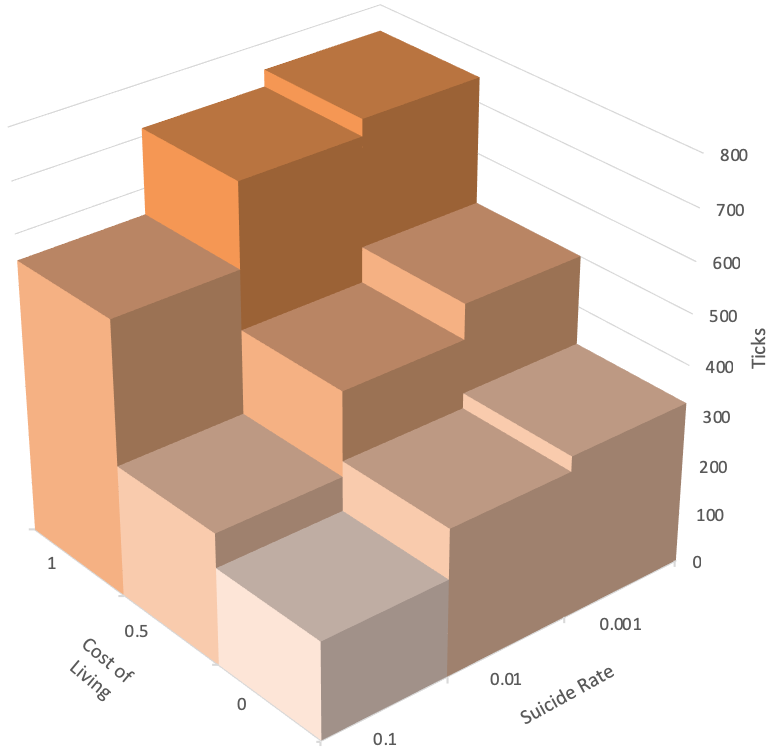
\includegraphics[scale=0.6]{figures/3d_histogram.png}
\caption{Implications of \textit{altruistic suicide} rates}
\label{fig:3d-histogram} 
\end{figure}

\begin{flushleft}
todo
\end{flushleft}

%%%%%%%%%%%%%%%%%%%%%%%%%%%%%%%%%%%%%%%%%%%%%%%%%%%%%%%%%%%%%%%%%%%%%%%%
%%%%%%%%%%%%%%%%%%%%%%%%%%%%%%%%%%%%%%%%%%%%%%%%%%%%%%%%%%%%%%%%%%%%%%%%
%%%%%%%%%%%%%%%%%%%%%%%%%%%%%%%%%%%%%%%%%%%%%%%%%%%%%%%%%%%%%%%%%%%%%%%%































\section{Discussion}
\begin{flushleft}
Results clearly show that the time to reach maximum population increases when:
\end{flushleft}
\begin{itemize}
\item \textit{Suicide Rate} decreases (more selfish)
\item \textit{Cost of Living} increases (harsh conditions)
\end{itemize}
\begin{flushleft}
Of course there is a limit to how much \textit{altruistic suicide} contributes to growth. But this is not reflected by this simulation for even high suicide rates; the reason for this is intrinsic to the logic of the simulation rules, but this is a different story that will not be addressed in this report.
\end{flushleft}

\begin{flushleft}

\end{flushleft}

\begin{flushleft}

\end{flushleft}

\begin{flushleft}

\end{flushleft}

%%%%%%%%%%%%%%%%%%%%%%%%%%%%%%%%%%%%%%%%%%%%%%%%%%%%%%%%%%%%%%%%%%%%%%%%
%%%%%%%%%%%%%%%%%%%%%%%%%%%%%%%%%%%%%%%%%%%%%%%%%%%%%%%%%%%%%%%%%%%%%%%%
%%%%%%%%%%%%%%%%%%%%%%%%%%%%%%%%%%%%%%%%%%%%%%%%%%%%%%%%%%%%%%%%%%%%%%%%

\section{Conclusion}
\begin{flushleft}

\end{flushleft}

%%%%%%%%%%%%%%%%%%%%%%%%%%%%%%%%%%%%%%%%%%%%%%%%%%%%%%%%%%%%%%%%%%%%%%%%
%%%%%%%%%%%%%%%%%%%%%%%%%%%%%%%%%%%%%%%%%%%%%%%%%%%%%%%%%%%%%%%%%%%%%%%%
%%%%%%%%%%%%%%%%%%%%%%%%%%%%%%%%%%%%%%%%%%%%%%%%%%%%%%%%%%%%%%%%%%%%%%%%

\raggedright
\bibliographystyle{apalike}
\bibliography{bibliography}

\end{document}
